\chapter{ به‌کارگیری تی‌اس‌ان‌ای بر روی مجموعه داده‌های بزرگ}
%%%%%%%%%%%%%%%%%%%%%%%%%%%%%%%%%%%%%%%%%%%
\section*{جمع‌بارگیری تی‌اس‌ان‌ای بر روی مجموعه داده‌های بزرگ}
مانند بسیاری دیگر از تکنیک‌های مصورسازی داده، تی‌اس‌ان‌ای از نظر پیچیدگی زمان و حافظه به نسبت تعداد داده‌های درجه 2 است. این امر باعث می‌شود تا اعمال این الگوریتم بر روی‌مجموعه داده‌هایی که بیش از ۱۰۰۰۰ دارند غیر ممکن شود. مشخصا نمونه برداری از روی داده‌ها یک راه حل ممکن برای رفع این مشکل است؛ اما این روش نمی‌تواند از اطلاعاتی که داده‌های انتخاب نشده در نمونه برداری در مورد گوناگونی داده‌های دیتاست در اختیار ما می‌گذارند بهره ببرد. به عنوان مثال فرض کنید داده‌های
 $A$، $B$، $C$
  در فضای چند بعدی به صورت دو به دو فاصله‌ی یکسانی از یکدیگر داشته باشند. اگر تعداد زیادی داده‌ی نمایش داده نشده در بین $A$ و $C$ وجود داشته باشد اما تمام داده‌های بین $A$ و $B$ در نمونه برداری موجود باشند، آنگاه احتمال اینکه $A$ و $B$ بخشی از یک خوشه باشند بسیار بیش‌تر از احتمال هم خوشه بودن $A$ و $C$ است. این امر در \cref{chapfig3} نشان داده شده است. در این بخش نشان خواهیم داد که تی‌اس‌ان‌ای چگونه می تواند تغییر کند تا با نشان دادن یک زیرمجموعه تصادفی از داده‌ها بتواند از تمام اطلاعات مربوط به تنوع داده‌های دیتاست اصلی استفاده نماید.
\\

\begin{figure}
	\centering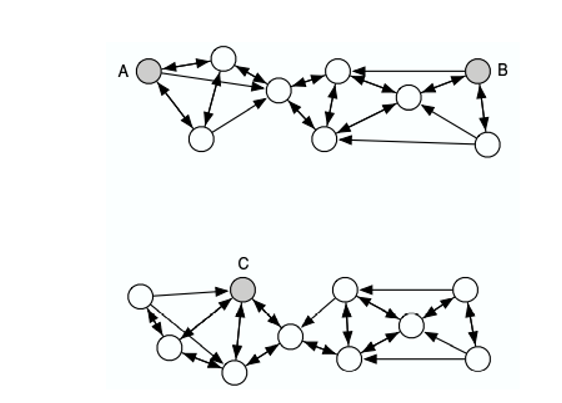
\includegraphics[scale=.6]{chapfig3.PNG}
	\caption{ }\label{chapfig3}
\end{figure}
\begin{figure}
	\centering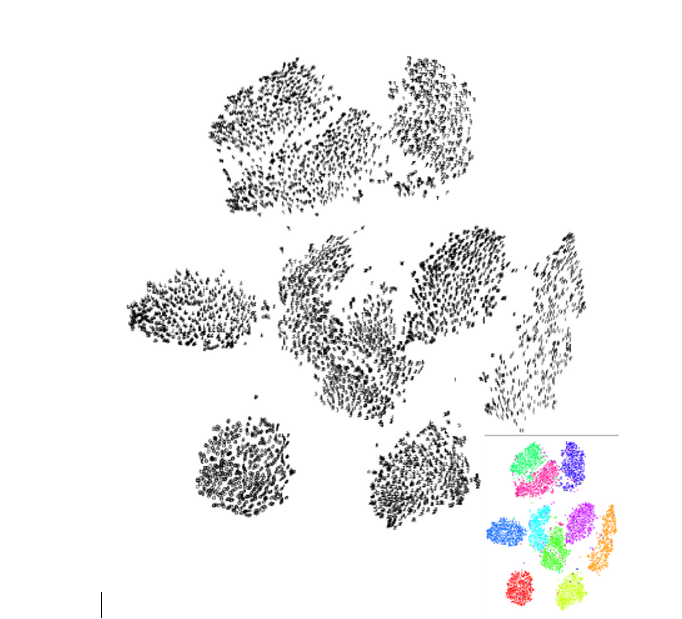
\includegraphics[scale=.6]{chapfig2.PNG}
	\caption{ }\label{chapfig2}
\end{figure}


به کارگیری تی‌اس‌ان‌ای بر روی مجموعه داده‌های بزرگ
برای این‌ کار، ابتدا یک تعداد مشخص از نقاط همسایه را در نظر می‌گیریم و یک گراف همسایگی برای تمام داده‌ها می‌سازیم. اگرچه این کار بار محاسباتی بسیار زیادی دارد، اما قرار است تنها یک بار این فرایند را انجام دهیم. سپس از هر نقطه برجسته ، به طور تصادفی شروع به قدم زدن بر روی گراف همسایگی می‌کنیم تا به یک نقطه برجسته دیگر برسیم. در حین قدم زدن تصادفی، احتمال انتخاب هر یال که از نقطه
 $x_i$
  شروع و به نقطه $xj$ ختم می‌شود، متناسب است با
$e^{‖x_i-x_j ‖^2}$
. مقدار
$ P_{j|i}$
 برابر است با بزرگی نسبی تعداد قدم‌های تصادفی که از نقطه‌ی برجسته‌ی$ x_i$ شروع شده وبه نقطه‌ی برجسته‌ی$ x_j$ ختم می‌شود. این تعریف شباهت‌هایی با روش $Isomap$ دارد که شباهت دو به دوی نقاط را اندازه‌گیری می‌کند. با این حال، همانند نقشه‌های انتشار، به جای اینکه به دنبال کوتاه ترین مسیر در گراف همسایگی باشیم، مقیاس نزدیکی بر مبنای قدم زدن تصادفی برای تمام مسیرها با یکدیگر ادغام می‌شوند. بنابراین، مقیاس نزدیکی بر مبنای قدم زدن تصادفی، در برابر مسیرهای کوتاهی که توسط داده‌های نویز ساخته شده‌اند یعنی $"short circuiting"$مقاوم است. (تعدادی داده‌ی نویز می‌توانند یک مسیر کوتاه بین دو خوشه جدا از هم بسازند که باعث متصل شدن دو خوشه می‌شود.)


بدیهی ترین روش برای محاسبه میزان شباهت بر مبنای قدم زدن تصادفی این است که به طور مستقیم قدم زدن تصادفی را بر روی گراف همسایگی اجرا کنیم که این روش در عمل بسیار کابردی است، چراکه می‌توان در هر ثانیه حدود یک میلیون بار قدم زدن را اجرا کرد. در روشی دیگر، یک راه حل تحلیلی برای محاسبه‌ی دو به دوی شباهت‌ها ارائه می‌شود که شامل حل کردن یک مدل خطی غیر متراکم است.  در تجربه‌های اولیه، چندان تفاوتی میان اجرای مستقیم قدم زدن تصادفی و روش‌های تحلیلی مشاهده نمی‌‌شود. در آزمایشی که در این بخش به آن می‌پردازیم، برای محاسبه شباهت‌ها به اجرای مستقیم قدم زدن تصادفی روی می‌آوریم چراکه بار محاسباتی کمتری دارد. اما در نظر داشته باشید که برای دیتاست‌های بسیار بزرگ که ممکن است نقاط استراژیک بسیار پراکنده باشند، روش‌های تحلیلی کارآمد تر خواهند بود. \cref{chapfig2} نتیجه یک آزمایش را نشان می‌دهد که در آن برای محاسبه دو به دوی شباهت‌ها، قدم زدن تصادفی را بر روی یک مجموعه‌ی شش هزارتایی از داده‌ها که به طور تصادفی از میان یک دیتاست شصت هزارتایی انتخاب شده‌اند اجرا شده است. در این آزمایش، از یک گراف همسایگی استفاده شده است که به ازای مقدار $K=20$ ساخته می‌شود؛ یعنی بیست تا از نزدیکترین همسایه‌های هر نقطه انتخاب می‌شوند. قسمت داخلی شکل، کل دیتاست را نشان می‌دهد که هر کلاس با یک رنگ خاص و متفاوت نشان داده شده است. در نقشه تی‌اس‌ان‌ای کاملا می‌توان مشاهده کرد که کلاس‌های مختلف به خوبی از یکدیگر قابل تفکیک می‌باشند و علاوه بر آن، واریانس و شکل خوشه‌ها به خوبی حفظ شده است. عملکرد بسیار خوب   تی‌اس‌ان‌ای را می‌توان از خطای تعمیم  \LTRfootnote{generalization error} محاسبه شده برای الگوریتم $KNN$ نیز مشاهده کرد. در حالیکه خطای تعمیم برای الگوریتم $KNN$ به ازای $K=1$ که بر روی دیتاست اصلی آموزش دیده است برابر 5.75 درصد است، مقدار این خطا برای همین الگوریتم که بر روی دیتاست‌ای که توسط تی‌اس‌ان‌ای تولید شده است آموزش دیده، برابر 5.13 درصد است. بار محاسباتی برای اجرای قدم زدن تصادفی تی‌اس‌ان‌ای بسیار معقول است. به طوریکه تنها یک ساعت زمان برای تولید \cref{chapfig2} لازم است.

